\documentclass[10pt,a4paper]{article}
\usepackage[utf8]{inputenc}
\usepackage{amsmath}
\usepackage{amsfonts}
\usepackage{amssymb}
\usepackage{makeidx}
\usepackage{graphicx}
\usepackage[left=2cm,right=2cm,top=2cm,bottom=2cm]{geometry}
\author{Miguel Angel Xamie Diaz Fuentes/Jimenez Cortes Raul}

\begin{document}
\begin{center}
\begin{LARGE}
\textbf{INGENIERÍA MECATRÓNICA}\\
\end{LARGE}
{\large Sistemas Eletrónicos De Interfaz}\\
\begin{figure}[hbtp]
\centering

\includegraphics[scale=0.80]{UPZMG_Mecatr_nica.png}
\end{figure} 
\begin{center}
\begin{LARGE}
EV-1-2-OPTOACOPLADORES Y RELEVADORES
\end{LARGE}
\end{center}

\begin{Large}
\textbf{Alumnos}
\\\textit{Miguel Angel Xamie Diaz Fuentes\\Raul Jimenez Cortez}
\textbf{\\Maestro}
\\\textit{Morán Garabito Carlos Enriquez}
\textbf{\\Fecha de Entrega}
\\\textit{03/10/2019}
\textbf{\\Grupo}
\\\textit{4-B}
\end{Large}

\end{center}

\footnote{Universidad Politécnica De La Zona Metropolitana De Guadalajara} 

\newpage

\section{Objetivo}

\begin{flushleft}
Integrar un sistema básico de control implementando sus etapas de interfaz de entrada, control e interfaz de salida.

\section{Materiales}

\begin{itemize}

\item Resistencias.
\item Relevadores.
\item Fuentes de Poder.
\item Multímetro.
\item Arduino.
\item Cables Duponk.
\item OptoAcopladores(425).
\item Led's.
\item Protoboards.
\item Transistores(2N2222).

\end{itemize}
\end{flushleft}
\section{Marco Teórico}

Un \textbf{OptoAcoplador}, también llamado \textbf{optoaislador} o \textbf{aislador acomplado ópticamente}, es un dispositivo de emisión y recepción que funciona como interruptor activado mediante luz emitida por un diodo led que satura un componente optoelectrónico, normalmente en forma de fototransistor o foto triac. De este modo se combinan en un solo dispositivo semiconductor, un foto emisor y un foto receptor cuya conexión entre ambos es óptica. Estos elementos se encuentran dentro de un encapsulado que por lo general es del tipo DIP. Se suelen utilizar para aislar eléctricamente a dispositivos muy sensibles.\\


Si la tensión de entrada varía, la cantidad de luz también lo hará, lo que significa que la tensión de salida cambia de acuerdo con la tensión de entrada. De este modo el dispositivo puede acomplar una señal de entrada con el circuito de salida, aunque hay que tener en cuenta que las curvas tensión/luz de led no son líneales, por lo que la señal puede distorsionarse. Se venden optoacompladores especiales para este propósito, diseñados de forma que tengan un rango en el que la señal de salida sea casi idéntica a la de la entrada.
\\

La función del circuito es como un PLC básico. Un \textbf{PLC o controlador lógico programable} es un dispositivo electrónico utilizados para controlar de forma automática distintos procesos o maquinas.\\
Estos PLC son computadoras capaces de automatizar procesos electromecánicos. Son muy utilizados en muchas industrias y maquinas. Estas computadoras son de fácil manejo por el operador, robustas, flexibles y económicas. Básicamente un PLC es capaz de ejecutar una acción (por ejemplo, accionar un motor) dependiendo de la señal que reciba de otro proceso.


\footnote{Universidad Politécnica De La Zona Metropolitana De Guadalajara} 
\newpage

\section{Desarrollo}

Primero se realizo el circuto de acuerdo al diagrama dado por el profesor el cual consta de 3 partes. La primera es la interfaz de entrada en el cual tenemos los optoacopladores realizando la función de interruptor con una entrada de 12v. En la segunda parte tenemos el control dado por el arduino y por ultimo tenemos el de interfaz de salida.\\

La estructura del circuito en diagrama es la siguiente:\\

\begin{figure}[hbtp]
\centering
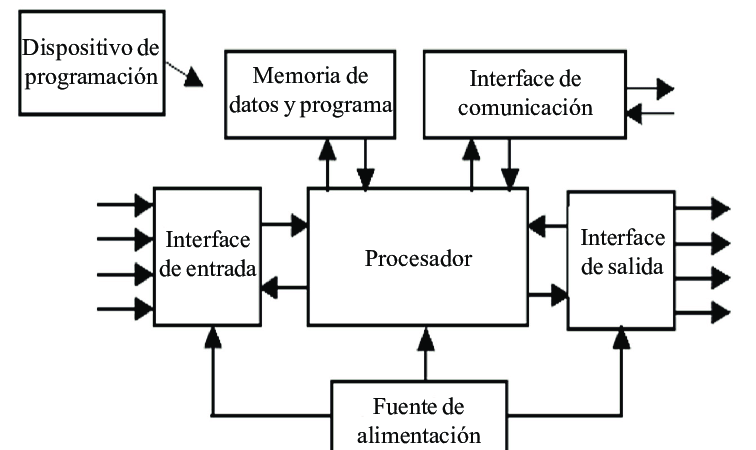
\includegraphics[scale=0.60]{estructura.png} 
\end{figure}

Para el uso de las resistencias correctas se realizaron calculos de acuerdo al modelo del optoacomplador y una que esta en función de salida hacia el arduino y la recibe el transistor (2N2222).\\
Datos:\\

Voltajes de entrada: 12v, 5v.\\

Datos del optoacoplador:\\

If = 10mA ------
Vf = 1.12v\\

{\Large $ R_{Led} = {\Large \frac{(12v - 1.15v)}{10mA}}$} \\Aqui se toman los parametros del optoacoplador (425).\\

{\Large $R_{Led} = 1.085\Omega$}\\

{\Large $R_{Transistor} = \frac{(5v - 0.6v)*250}{12mA}$}\\ Aqui se toman los parametros del relevador y de la medida del transistor con el multimetro.\\

{\Large $R_{Transistor} = 1.528K\Omega$}\\

\footnote{Universidad Politécnica De La Zona Metropolitana De Guadalajara}
\newpage

Por ultimo también determinamos la potencia.\\

$ W = I^2 R $\\ 

$ W = (10mA)(1.100\Omega)$\\

$ W = 0.11w $\\

Para la segunda parte observamos el diagrama del circuito y lo conectamos al protoboard.

\begin{figure}[hbtp]
\centering
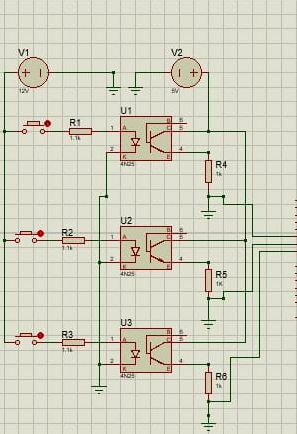
\includegraphics[scale=0.60]{entrada.png} 
\end{figure}

Algo muy importante es que como es un PLC se puede medir por partes, porque cada una es independiente asi que en esta parte medimos que reciba voltaje de entrada al presionar el boton y que haga contacto con el tierra cerrando el circuito, se midio con el multimetro y daba 1.17v al presionar el boton, luego se mide que al presionar el boton el receptor haga su función cerrando el interruptor al detectar la emisión dando 5v en el pin que esta con la resistencia a tierra, aqui sera tu pin emisor hacia el control.

\begin{figure}[hbtp]
\centering
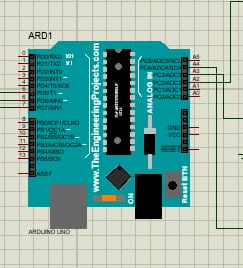
\includegraphics[scale=0.60]{arduino.png} 
\end{figure}


\footnote{Universidad Politécnica De La Zona Metropolitana De Guadalajara}

\newpage

En la parte de control tenemos el código el cual debe realizar  la función que al recibir la señal esta genera una salida positiva (5v) la cual activara los relevadores o led's dependiendo la necesidad del usuario, en este caso ambas.\\
\begin{figure}[hbtp]
\centering
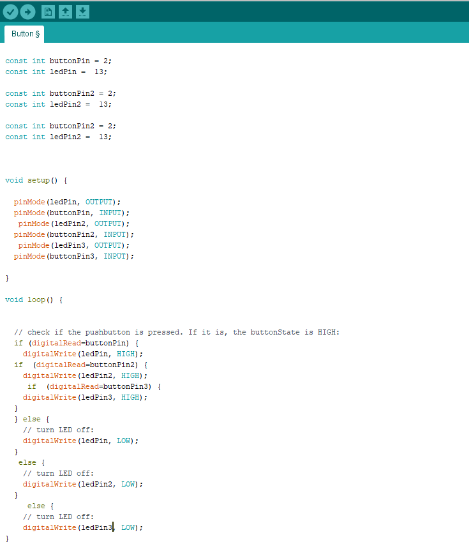
\includegraphics[scale=0.40]{codigo.png} 
\end{figure}

Luego tenemos la interfaz de salida la cual al recibir los 5v en la resistencia que va hacia la base del transistor este también hace la funcion de un interruptor al detectar voltaje permite el paso entre el emisor y el receptor cerrando asi el circuito y encendiendo el led o apagandolo. Para comprobar esta parte fue necesario revisar los relevadores viendo que esten en perfecto funcionamiento y también la resistencia del transistor. A continuación tenemos el diagrama.

\begin{figure}[hbtp]
\centering
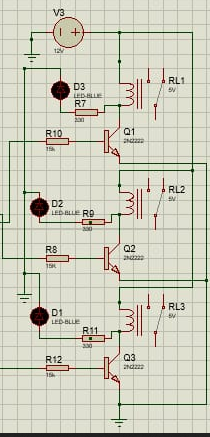
\includegraphics[scale=0.60]{salida.png} 
\end{figure}

\footnote{Universidad Politécnica De La Zona Metropolitana De Guadalajara}
\newpage
Cuando se prueba cada parte de las interfaces se realiza la conexión debida y revisando que no se realize un falso contacto con algunos de los cables de entrada o con las resistencias.\\ \textbf{A continuación tenemos las evidencias del circuito.}


\begin{figure}[hbtp]
\centering
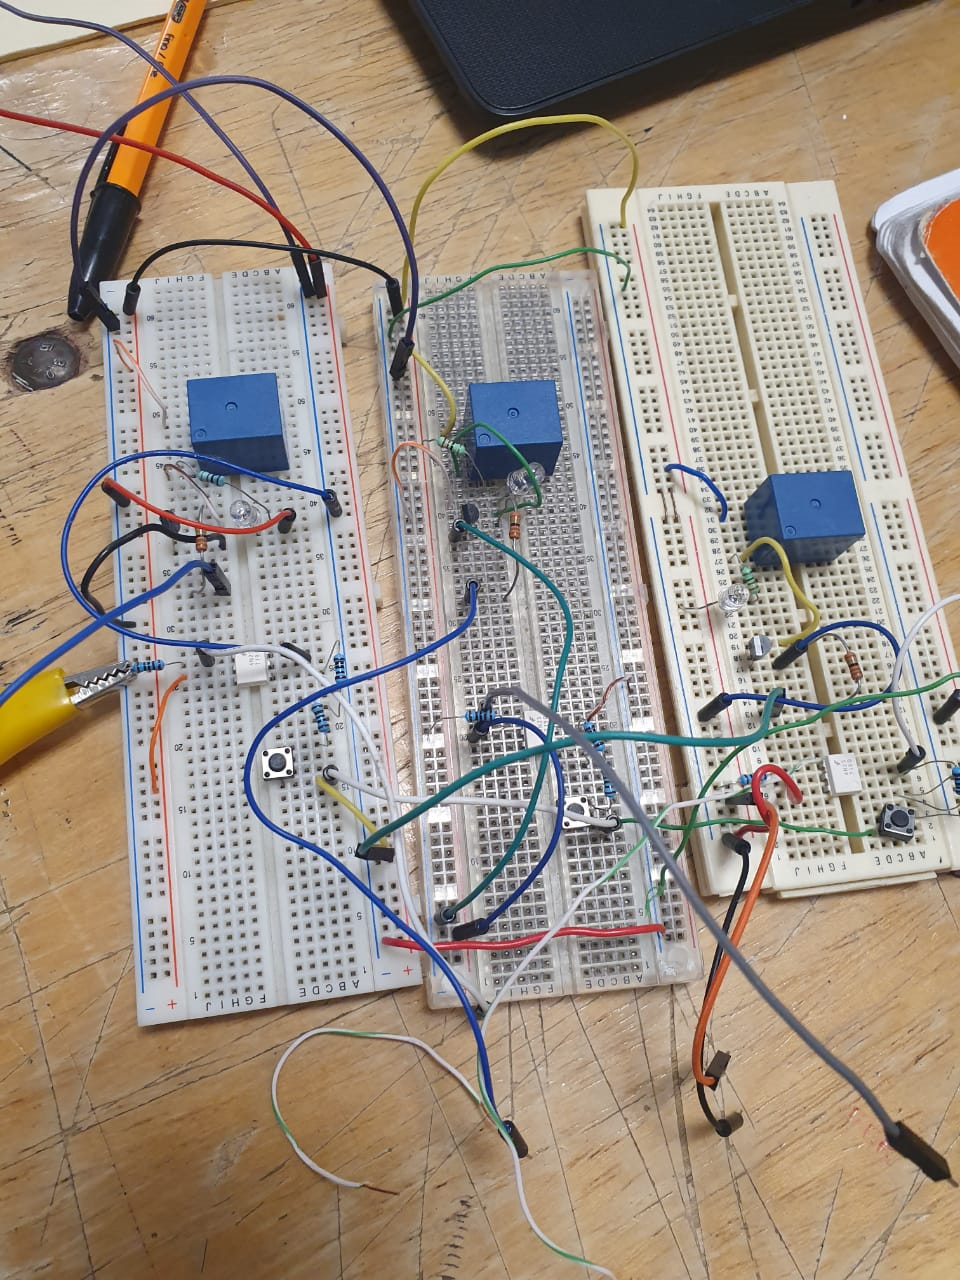
\includegraphics[scale=0.30]{001.png} 
\end{figure}

\footnote{Universidad Politécnica De La Zona Metropolitana De Guadalajara}
\newpage
Aqui podemos observar el circuito encendido en su totalidad.
\begin{figure}[hbtp]
\centering
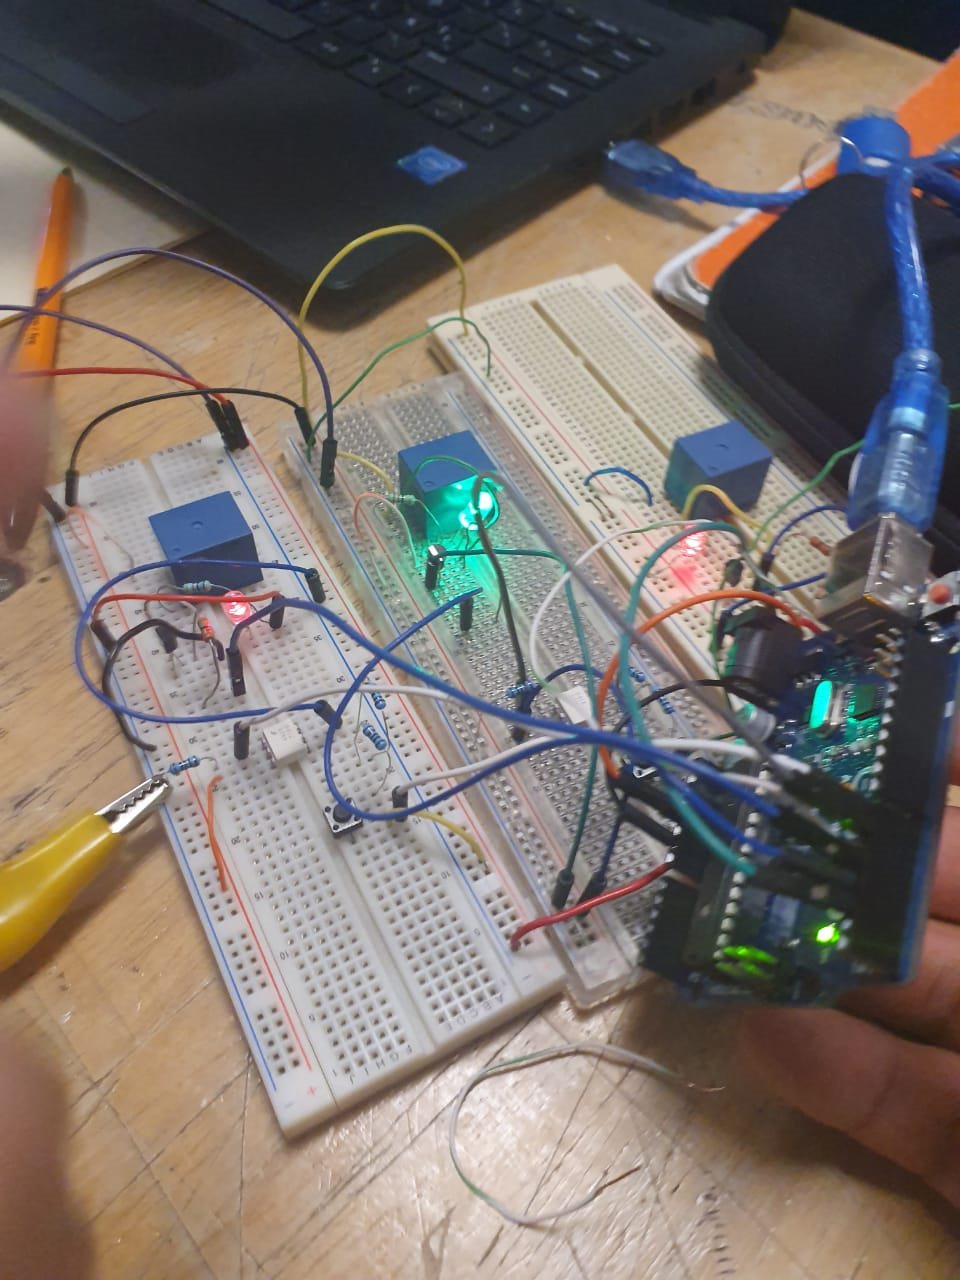
\includegraphics[scale=0.30]{002.png} 
\end{figure}\\
Presionando una entrada.
\begin{figure}[hbtp]
\centering
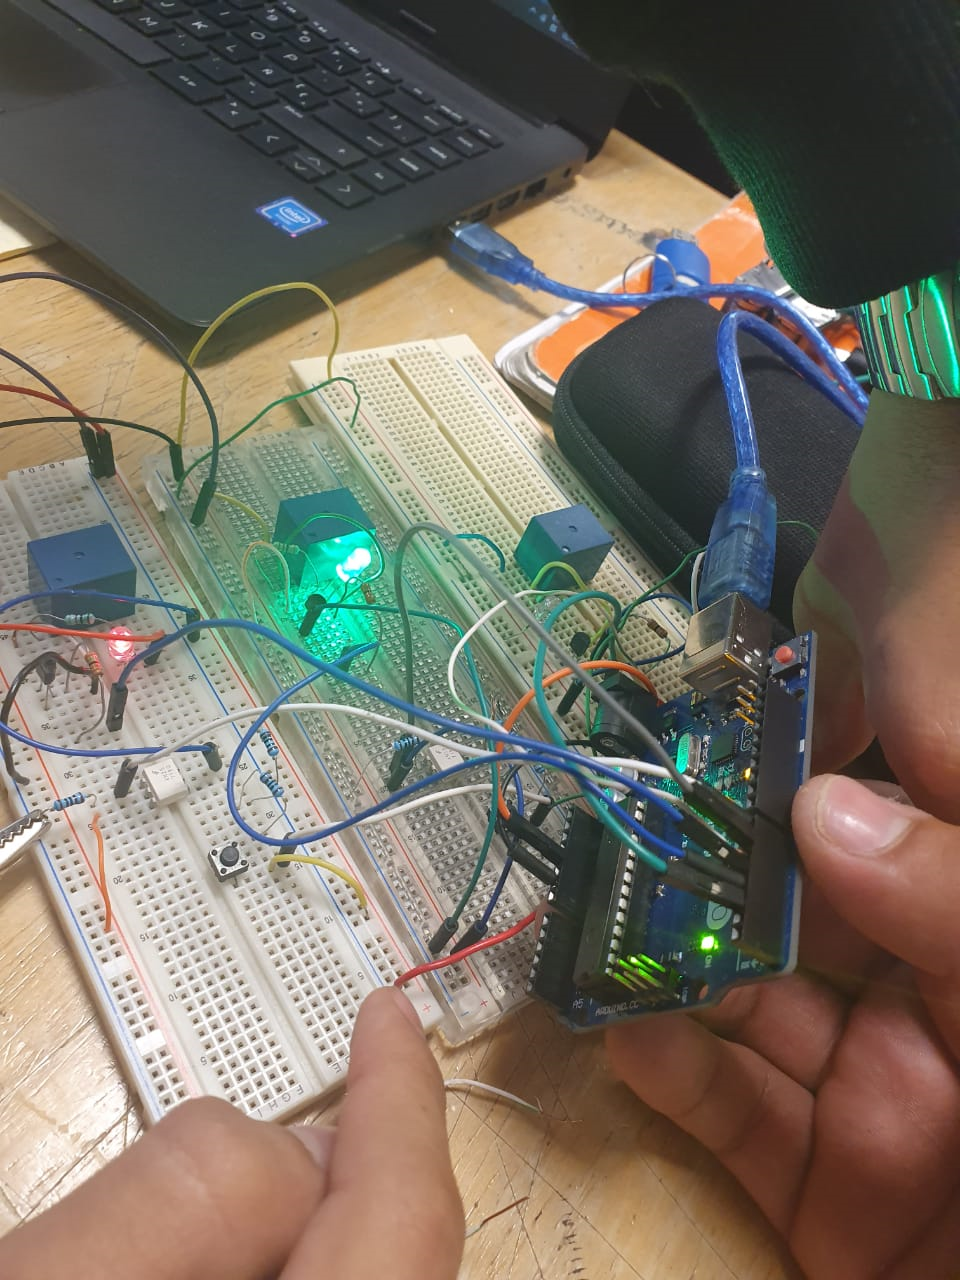
\includegraphics[scale=0.25]{003.png} 
\end{figure}

\footnote{Universidad Politécnica De La Zona Metropolitana De Guadalajara}
\newpage

Presionando la segunda entrada.
\begin{figure}[hbtp]
\centering
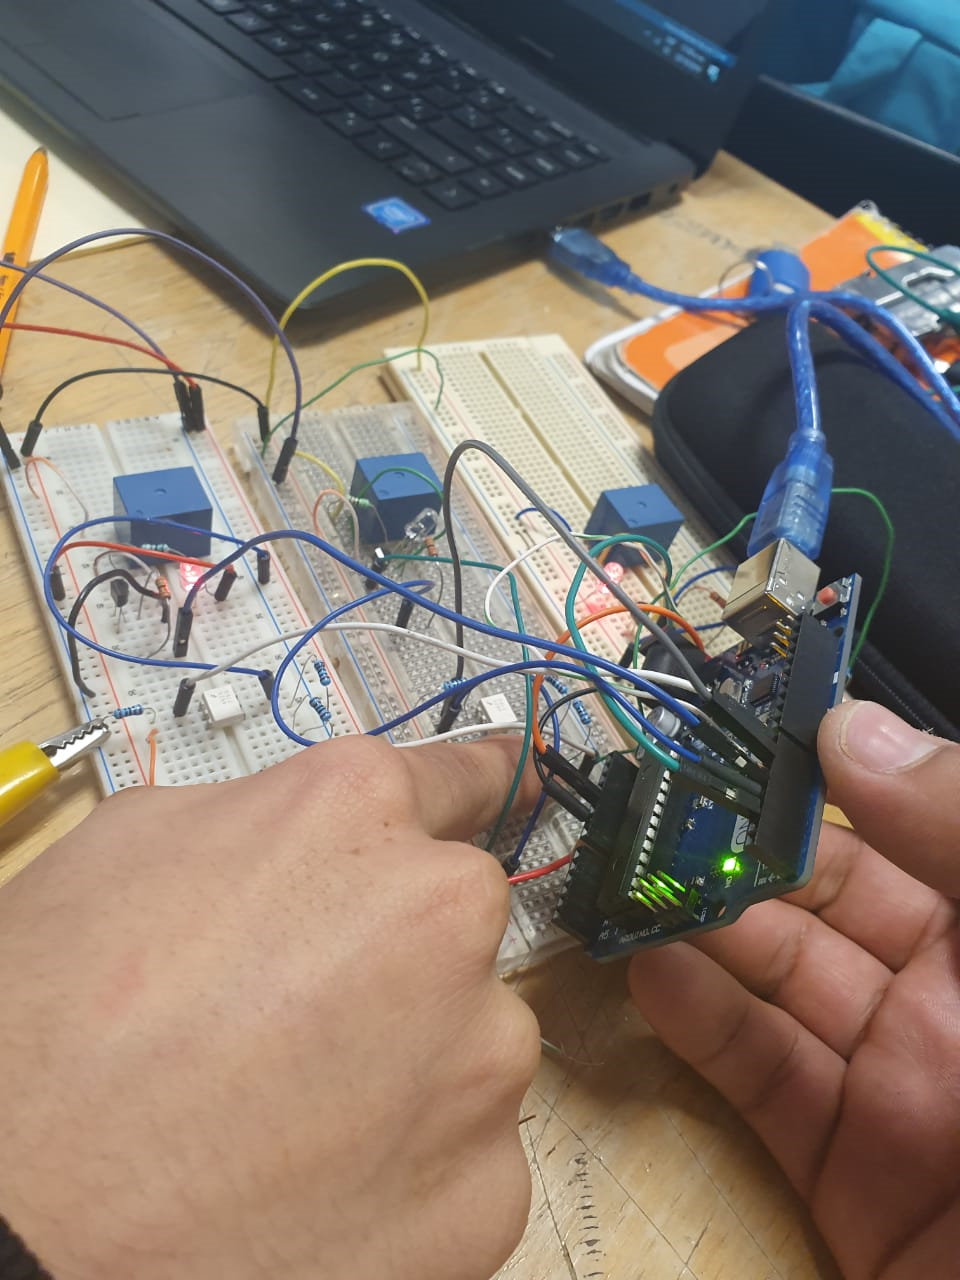
\includegraphics[scale=0.27]{004.png} 
\end{figure}\\
Presionando la ultima entrada.
\begin{figure}[hbtp]
\centering
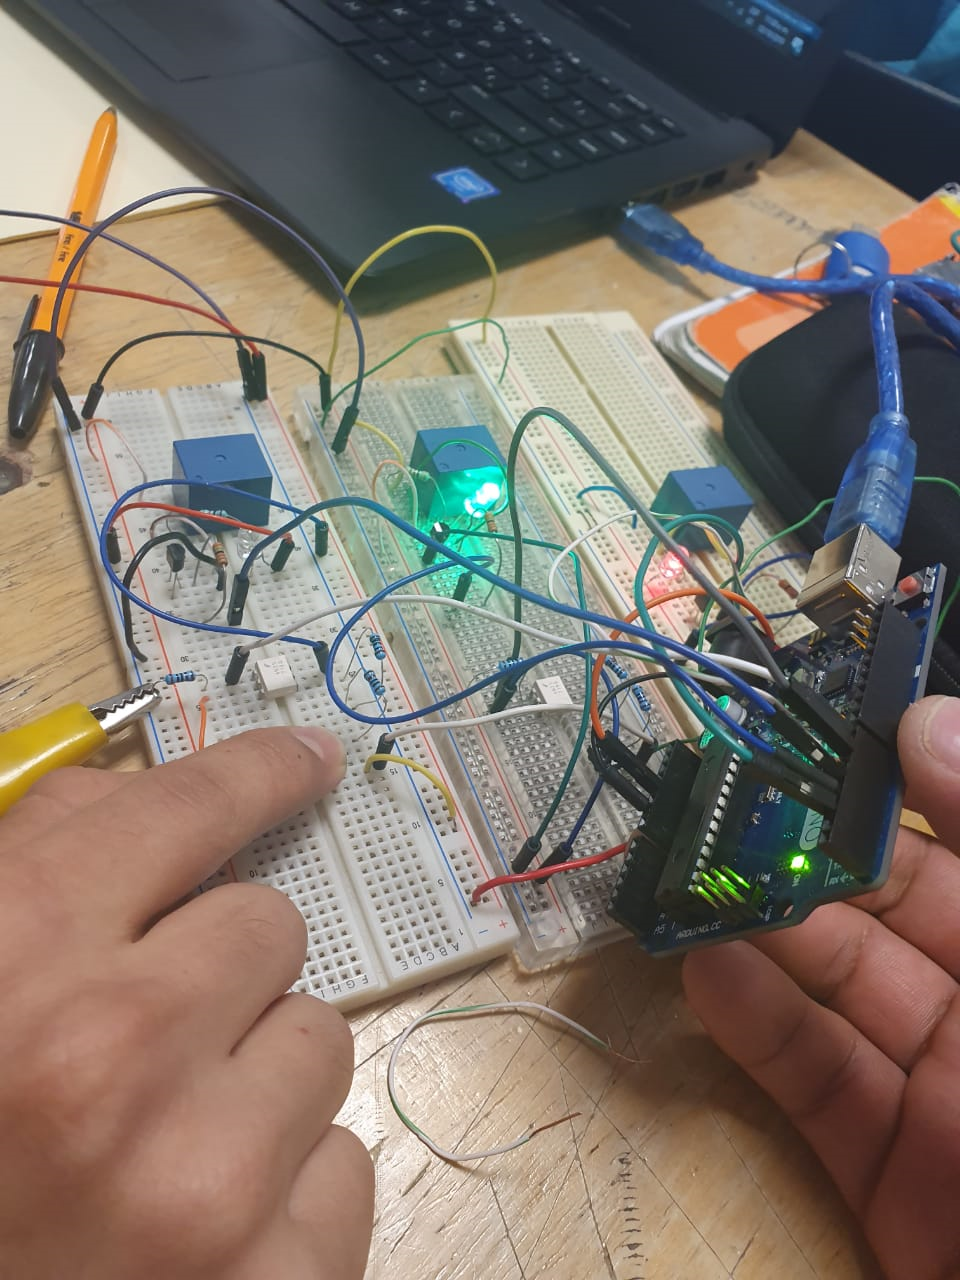
\includegraphics[scale=0.27]{005.png} 
\end{figure}
\footnote{Universidad Politécnica De La Zona Metropolitana De Guadalajara}
\newpage
\section{Conclusión}
En esta practica se pudo entender el funcionamiento el cual haría un PLC y a su vez la estructura en la que se comformó este mismo para la aplicación en este circuito ya que esta tambien se utiliza mucho en areas industriales. También con base al desarrollo, en la parte de los optoacopladores al ser un componente nuevo que utilize e no antes vitos en culquier otra practica junto con su funcionamiento ya que su estructura es parecida a un relevador pero con características distintas que me permitio saber como manipularlos y utilizarlos, lo más importante fue el saber como calcular las resistencias adecuadas para un circuito al utilizar este material y también la resistencia para transistores o relevadores, revisando su datasheet correspondiente con sus parametros necesarios para realizar estos calculos ya que conlleva todo a la pracica e se logro la obtencion de los resultados en los calculos como en la parte del circuito en fisico.

\bibliography{Referencia}
\begin{thebibliography}{X}
\bibitem{Baz} \textsc{MALVINO, ALBERT PAUL} \textit{Principios de Electrónica.} McGraw-Hill/Interamericana de España,S. A. U. 2000.

\bibitem{Baz} \textsc{M.A. LAUGHTON, D. J. WARNE (ED).} \textit{Electrical Engineer's.} 
Reference book, 16th edition,Newnes, 2003 Chapter 16 Programmable Controller.


\bibitem{Baz} \textsc{ALLEY-ATWOOD.} \textit{Ingeniería Electrónica.} 
ISBN 968-18-0967-X
\end{thebibliography}

\bibliographystyle{plain}
\footnote{Universidad Politécnica De La Zona Metropolitana De Guadalajara}
\end{document}